\documentclass[letterpaper, 10 pt, conference]{ieeeconf}  % Comment this line out if you need a4paper

%\documentclass[a4paper, 10pt, conference]{ieeeconf}      % Use this line for a4 paper

\IEEEoverridecommandlockouts                              % This command is only needed if 
                                                          % you want to use the \thanks command

\overrideIEEEmargins                                      % Needed to meet printer requirements.

%In case you encounter the following error:
%Error 1010 The PDF file may be corrupt (unable to open PDF file) OR
%Error 1000 An error occurred while parsing a contents stream. Unable to analyze the PDF file.
%This is a known problem with pdfLaTeX conversion filter. The file cannot be opened with acrobat reader
%Please use one of the alternatives below to circumvent this error by uncommenting one or the other
%\pdfobjcompresslevel=0
%\pdfminorversion=4

% See the \addtolength command later in the file to balance the column lengths
% on the last page of the document

% The following packages can be found on http:\\www.ctan.org1
%\usepackage{graphics} % for pdf, bitmapped graphics files
%\usepackage{epsfig} % for postscript graphics files
%\usepackage{mathptmx} % assumes new font selection scheme installed
%\usepackage{times} % assumes new font selection scheme installed
%\usepackage{amsmath} % assumes amsmath package installed
%\usepackage{amssymb}  % assumes amsmath package installed

\title{\LARGE \bf
Knowledge Graph Embedding in Multi-Agent Systems: A Distributed Control Perspective
}


\author{Sang-Won Kang${}^{1}$ and Hyo-Sung Ahn${}^{1*}$% <-this % stops a space
\thanks{*This work was not supported by any organization}% <-this % stops a space
\thanks{$^{1}$ School of Mechanical Engineering, Gwangju Institute of Science and Technology (GIST), Gwangju, Korea. 
        {\tt\small tony9707@gm.gist.ac.kr; hyosung@gist.ac.kr}}%
}

\usepackage{diagbox}
\usepackage{subcaption}
\usepackage{siunitx} % For units in tables
\usepackage[bottom]{footmisc}
\usepackage{physics}
\usepackage{amsmath,amsfonts,amssymb}
\newtheorem{theorem}{Theorem}[section]
\newtheorem{corollary}{Corollary}[theorem]
\newtheorem{lemma}[theorem]{Lemma}
\usepackage{graphicx}
\usepackage{tikz}
\usetikzlibrary{positioning, arrows}
%\usetikzlibrary{arrows.meta}
\tikzset{mynode/.style={draw, very thick, circle, minimum size=1cm},
    myarrow/.style={very thick, -Triangle}}



\begin{document}

\maketitle

\thispagestyle{empty}
\pagestyle{empty}

%%%%%%%%%%%%%%%%%%%%%%%%%%%%%%%%%%%%%%%%%%%%%%%%%%%%%%%%%%%%%%%%%%%%%%%%%%%%%%%%
\begin{abstract}
This paper proposes a novel framework that integrates Knowledge Graph Embedding (KGE) with distributed optimization and formation control in multi-agent systems. By focusing on TransE, we reformulate its optimization problem using the in-degree Laplacian matrix and distributed control theory, allowing agents to represent entities in the knowledge graph and interact only with neighboring entities. This framework offers a new perspective on embedding methods in decentralized environments and provides a foundation for future research in applying formation control to complex network structures. 
\end{abstract}


%%%%%%%%%%%%%%%%%%%%%%%%%%%%%%%%%%%%%%%%%%%%%%%%%%%%%%%%%%%%%%%%%%%%%%%%%%%%%%%%
\section{Introduction}
Knowledge Graph Embedding (KGE) has emerged as a powerful method for representing entities and relations in a continuous vector space. By embedding knowledge graphs, various downstream tasks such as link prediction, entity classification, and relation extraction are greatly enhanced \cite{wang_knowledge_2017}. Among the KGE techniques, TransE \cite{bordes_translating_2013} is one of the most popular and simplest methods, where relations between entities are modeled as translations in the embedding space. Despite its simplicity, TransE has performed remarkably in various knowledge graph tasks.

However, as the size and complexity of knowledge graphs grow, it becomes important to distribute the learning process among multiple agents, especially when dealing with decentralized or multi-agent systems. In such cases, traditional centralized optimization techniques may not be feasible. To address this, distributed optimization methods have gained significant attention in recent years. Distributed optimization allows each agent to focus on local objectives while collectively contributing to the global solution \cite{yang_survey_2019}. This makes it suitable for scenarios where agents have limited knowledge of the global network.

In this work, we propose a novel approach that connects TransE with distributed optimization and formation control. Our main result indicates how the TransE optimization problem can be formulated as a distributed optimization problem, where agents only interact with their neighbors. Furthermore, we demonstrate that the system's convergence can be analyzed using graph-theoretical tools, particularly the properties of the graph Laplacian. By drawing parallels with formation control in multi-agent systems, we establish a framework for understanding the dynamics of embedding in multi-agent settings.

The remainder of this paper is structured as follows: Section 2 provides the necessary preliminaries on graph theory and the TransE model. Section 3 presents our main results, illustrating the correspondence between KGE and formation control through both theoretical analysis and simulation. Finally, Section 4 concludes the paper with a discussion of the implications of our findings and potential directions for future research.

\section{Preliminaries}
This section introduces the essential concepts and mathematical tools that underpin our main results. We cover the basics of TransE, distributed optimization, and formation control, which will be used to derive our conclusions in the subsequent sections.

\subsection{Graph Theory}

Graph theory forms the foundation for modeling and analyzing the interactions and relationships in both knowledge graphs and multi-agent systems. In this work, we leverage graph theoretical concepts to unify the fields of Knowledge Graph Embedding (KGE) and formation control.

A \textbf{graph} \( G = (V, E) \) consists of a set of vertices \( V \) (or nodes) and a set of edges \( E \) that connect pairs of vertices. Each edge \( e \in E \) is an ordered pair \( (v_i, v_j) \), where \( v_i, v_j \in V \). In a \textbf{directed graph} (or digraph), edges have a direction, pointing from one vertex (the head) to another (the tail).

\subsubsection{Adjacency Matrix}

The \textbf{adjacency matrix} \( A \) of a graph \( G \) is a matrix where \( A_{ij} = 1 \) if there is a directed edge from vertex \( v_i \) to vertex \( v_j \), and \( A_{ij} = 0 \) otherwise. The adjacency matrix is crucial in representing the connectivity and structure of the graph, which directly impacts the behavior of vertices.

\subsubsection{Laplacian Matrix}

The \textbf{Laplacian matrix} \( L \) is derived from the adjacency matrix and plays a key role in understanding the graph's attributes \cite{mirzaev_laplacian_2013}. For a directed graph, the \textbf{in-degree Laplacian matrix} \( L \) is defined as:

\[
L = D - A
\]

\noindent where \( D \) is the diagonal matrix of in-degrees, with each diagonal element \( D(i, i) \) equal to the in-degree of vertex \( v_i \), the number of edges directed towards \( v_i \).

\noindent The Laplacian matrix is fundamental in analyzing the dynamics of multi-agent systems, particularly in formation control, where it governs how agents influence each other based on the underlying graph structure.

In our work, $L$ is used to describe the linear couplings between entities in the knowledge graph. By analyzing the eigenvalues and eigenvectors $L$, we can infer whether the system converges to a stable solution or diverges in the embedding space.

\subsection{TransE}
TransE \cite{bordes_translating_2013} is a popular method for knowledge graph embedding that represents entities as vectors in a continuous space. Let $\mathcal{G} = (\mathcal{E}, \mathcal{R})$ be a knowledge graph where $\mathcal{E}$ is the set of entities and $\mathcal{R}$ is the set of relations. Given a triple $(h, r, t)$, where $h \in \mathcal{E}$ is the head entity, $t \in \mathcal{E}$ is the tail entity, and $r \in \mathcal{R}$ is the relation, TransE embeds $h$, $r$, and $t$ as vectors in $\mathbb{R}^d$ such that:
\[
\mathbf{h} + \mathbf{r} \approx \mathbf{t}
\]
Here, $\mathbf{h}$, $\mathbf{r}$, and $\mathbf{t}$ are the embedding vectors of $h$, $r$, and $t$, respectively. The objective function to minimize is typically formulated as:
\[
L(\mathcal{G}) = \sum_{(h,r,t) \in \mathcal{G}} \|\mathbf{h} + \mathbf{r} - \mathbf{t}\|_2^2
\]

This energy function drives the model to learn embeddings where the relational structure is preserved in the vector space. 

\subsection{Distributed Optimization}
In a distributed optimization framework, we consider a network of $N$ agents, where each agent $i$ has access to a local objective function $f_i(x_i)$ and interacts only with its neighboring agents in a communication graph. The global optimization problem is given by:
\[
\min \sum_{i=1}^{N} f_i(x_i)
\]
Each agent aims to minimize its own objective while exchanging information with neighboring agents to achieve a global consensus \cite{nedic_distributed_2009}. Distributed optimization is well-suited for large-scale systems where centralized optimization is impractical due to communication or computational constraints.

In this work, we interpret the TransE objective function as a distributed optimization problem where each agent corresponds to an entity in the knowledge graph and interacts with its neighbors via relation-specific and uni-directed interactions. The goal of each agent is to minimize the local objective derived from the TransE energy function while collectively achieving an embedding that satisfies the global structure of the knowledge graph.

\subsection{Formation Control}
Formation control is a widely studied problem in multi-agent systems where the goal is to drive a group of agents to achieve and maintain a desired formation \cite{oh_survey_2015}. The control law typically depends on the relative positions of the agents and can be written as:
\[
\dot{x}_i = k_p\sum_{j \in \mathcal{N}_i} (x_i - x_j - d_{ji})
\]
where $x_i$ is the position of agent $i$, $\mathcal{N}_i$ is the set of neighbors of agent $i$, and $d_{ij}$ is the desired relative displacement between agents $i$ and $j$. $k_p$ is a negative proportional gain of control law. The dynamics ensure agents converge to a formation that satisfies the specified relative displacements.

In the context of TransE, we draw an analogy between formation control and distributed optimization. The update rule for each agent in the optimization process can be viewed as a control law that governs the motion of entities in the embedding space. By leveraging tools from formation control theory, we can analyze the stability and convergence of the embedding process.

\section{Main Result}

\subsection{TransE and Distributed Optimization}

TransE typically employs a margin-based energy function, but in this case, we reformulate the optimization problem for each agent's TransE in a graph as follows:
\begin{subequations}
\begin{equation}\label{eq:min}
    \min \sum_{i=1}^{N} f_{i} (x_{i})
\end{equation}
\begin{equation}\label{eq:f_i}
    f_{i}(x_{i}) = \sum_{j \in \mathcal{H}_{i}} \frac{1}{2} \|x_{i} - x_{j} - r_{ji}\|_{2}^{2}
\end{equation}
\end{subequations}
Here, \( x \ \in \mathbb{R}^{d \times N} \) represents entities, with \( x_i \in \mathbb{R}^d \) being the \(i\)th agent among \( N \) agents, and \( j \) denotes the neighbors of \( i \), which serve as the head entity and belong to the set \( \mathcal{H}_{i} \). \( r_{ji} \in \mathbb{R}^d \) represents a predefined relation vector from \( j \) to \( i \). 

The optimization problem \eqref{eq:min} is resolved by distributed optimization. Each agent focuses on its own objective function \eqref{eq:f_i}. % Despite their individual objectives, they can collectively achieve the global minimum through local optimization.
\begin{equation}
    p_i = - \pdv{f_{i}}{x_{i}} = - \sum_{j \in \mathcal{H}_i} (x_{i} - x_{j} - r_{ji})
    \label{eq:p}
\end{equation}
\( p_i \) is the steepest descent of \( f_i(x_i) \) toward a zero gradient used for Gradient Descent Method (GDM). Each \( x_i \) updates itself to reach settled state:
\begin{equation}
    x_{i}^{t+1} = x_i^t + \alpha p_i(x_i^t)
    \label{eq:update}
\end{equation}
\( \alpha \) is the step size regulating update speed of agents. Even though each agent may have own local minimum, determining the stabilization of the entire system is difficult. Therefore, we expand \( p_i \) into a vector form:
\begin{equation}
    p = - (Lx - r)
    \label{eq:p_vector}
\end{equation}

In this case, \( L \) represents the linear couplings between elements of \( x \), and \( r \) is a column vector containing all \( r_i \) (\( r_i = \sum_{j \in H_i} r_{ji} \)). Considering \eqref{eq:p_vector}, the original problem \eqref{eq:min} is reformulated as:

\begin{equation}
    \min \frac{1}{2} \|Lx - r\|_{2}^{2}
    \label{eq:new_min}
\end{equation}
\noindent The solution \( x^* \) of \eqref{eq:new_min} implies that \( Lx^* - r = 0 \). % when the objective function is convex. 

In summary, TransE for multi-agent graphs can be seen as an optimization problem that can be solved in a distributed manner. Furthermore, spectral properties of the graph Laplacian \( L \) allow us to analyze the overall system behavior.

\subsection{Formation Control with Displacement}

The matrix \( L \) has specific properties, particularly regarding its singularity, which affects the existence of \( x^* \). To verify the system’s convergence, we utilize a method from formation control theory. The update rule in GDM \eqref{eq:update} plays a crucial role. \eqref{eq:update} is reformulated as the \textbf{Euler method} of solving a differential equation with sufficently small time step $h$, \eqref{eq:dis_dynamic} where $k_p = h \alpha < 0$. 

%asdfasdfa

\begin{subequations}\label{eq:fc_law}
\begin{equation}\label{eq:dis_dynamic}
    \dot{x}_i = k_p \sum_{j \in \mathcal{H}_i} (x_{i} - x_{j} - r_{ji})
\end{equation}
\begin{equation}\label{eq:total_dynamic}
    \dot{x} = k_p(Lx - r)
\end{equation}
\end{subequations}

\eqref{eq:total_dynamic} is an expanded vector form of \eqref{eq:dis_dynamic}.

\noindent The dynamics in \eqref{eq:fc_law} represent a single integrator control law for displacement-based formation control of digraphs with a Laplacian matrix. As shown by the dynamics, the current state directly influences the rate of change. Thus, the previous distributed optimization problem and the new formation control problem are equivalent. Entities follow the control law \eqref{eq:fc_law}, making it possible to use control theory methods to analyze features of a new embedding system in continuous time.

Given the dynamics \eqref{eq:total_dynamic}, we can derive another equation:

\begin{equation}
    \ddot{x} = k_p L \dot{x}
    \label{eq:2dot}
\end{equation}

\noindent This differential equation has a simple solution:

\[
    \dot{x} = e^{k_p Lt} \dot{x}_0
\]

\noindent Since \( L \) is usually asymmetric and may have complex eigenvalues, we decompose \( L \) into Jordan form:

\[
    \dot{x} = Te^{k_p Jt}T^{-1} \dot{x}_0
\]

\noindent where \( L = TJT^{-1} \). The matrix \( L \) has some zero eigenvalues \( \lambda_n = 0 \indent (n = 1,2,...,M) \), and the real parts of the other nonzero eigenvalues are positive \cite{mirzaev_laplacian_2013}. As a result, the solution to \eqref{eq:2dot} approaches such a constant over time, where \( p_n \) and \( q_n \) are the left and right eigenvectors corresponding to \( \lambda_n \):

\begin{equation}
    \dot{x} \rightarrow (\sum_{n=1}^M q_n e^{-\lambda_n t}p_n^\top) \dot{x}_0 = (\sum_{n=1}^M q_n p_n^\top )\dot{x}_0
    \label{eq:solution}
\end{equation}

\noindent The equation \eqref{eq:solution} reminds us that $L$'s column and row null spaces critically impact multi-agent formation. 
To clarify it, we explore the shapes of the graphs that directly influence nullity of \( L\). We distinguish between two features of digraphs for KGE problems: \textbf{Stems} and \textbf{Cycles}.

A stem acts solely as head entities without being influenced by any external factors. For example, in Fig. \ref{fig:DAG}, the first entity is a stem node that influences the second and fourth nodes by enforcing the relation vectors \( r_{12} \) and \( r_{14} \). Since stems have no incoming edges, the Laplacian matrix \( L \) of graphs with \( m \) stem will have \( m \) zero rows. Consequently:
\[
    \dim \ker L \geq m
\]
If non-zero rows of $L$ are linearly independent, it exactly equals to $m$. 

Nodes within a cycle serve both as head and tail entities. Fig. \ref{fig:DCG} provides a good example of a triangular cycle. All rows of the Laplacian matrix \( L \) have a zero sum, resulting in \( L \) having a one-dimensional kernel. Additionally, the rows are linearly dependent because there are no zero rows.


Given these features, we organized several cases of graphs for knowledge graph embedding: \textbf{Acyclic Digraphs} and \textbf{Cyclic Digraphs}.

\subsubsection{Acyclic Digraphs}

We defined an acyclic digraph as having some stems. These stems will strongly stabilize embedding result. Moreover, in cases of acyclic digraph, zero multiplicity of $L$'s eigenvalues must equals to the number of stems. The following lemma then holds for acyclic digraphs.

\begin{lemma}\label{lemma:p}
Let the \( n \)-th row of \( L \) be a zero row. Then the null space of this row includes vectors of the form:
\begin{equation}\label{eq:DAG_left}
    p = \{0, \dots, 0, \rho_n = 1, 0, \dots, 0\}^\top
\end{equation}
\end{lemma}

\begin{proof}
Since the \( n \)-th row is a zero row, it is linearly dependent. Therefore, a vector \( p \) which satisfies \( p^\top L = \mathbf{0}_N^\top \) always exists.
\end{proof}

From Lemma \ref{lemma:p}, we concluded acyclic digraphs always converge.

\begin{theorem}\label{th:DAG_converge}
If an acyclic digraph satisfies Lemma \ref{lemma:p}, its embedding formation will converge to constant positions.
\end{theorem}

\begin{proof}
The stem nodes \( x_n \) experience no external forces, so \( \dot{x}_n = 0 \). Consequently:
\begin{equation}\label{eq:0_N}
    \dot{x} \rightarrow \sum_{n=1}^M q_n p_n^\top \dot{x}_0 = \sum_{n=1}^M (q_n \times 0) = \mathbf{0}_N
\end{equation}
\end{proof}


%Fig. \ref{fig:AG1} is another situation of the ayclic graph which consists of cycles and direct stems. 
%The node $E_3$ receives a force from $E_4$ then the rows of $L$ cannot keep linear dependence. That will generate a converging effect. 
%%%%%%%%%%%%%%%%%%%%%%%%%%%%%%%%%%%%%%%%%%%%%%%%%%%%%%%%%%%%%%%%%%%%%%%%%%%%%%%%%%%%
\begin{figure}[h] % 'h' specifies placement (here)
\centering
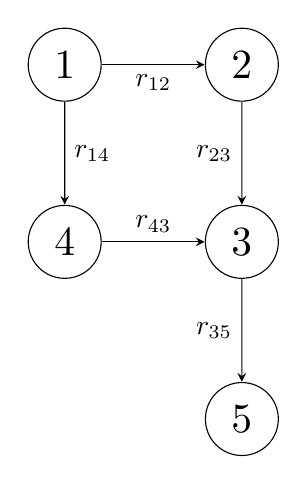
\begin{tikzpicture}[>=stealth, node distance=1.5cm]

% Define nodes
\node[circle, draw, fill=white!20, scale = 1.5] (1) {1};
\node[circle, draw, fill=white!20, scale = 1.5, right of=1] (2) {2};
\node[circle, draw, fill=white!20, scale = 1.5, below of=2] (3) {3};
\node[circle, draw, fill=white!20, scale = 1.5, left of=3] (4) {4};
\node[circle, draw, fill=white!20, scale = 1.5, below of=3] (5) {5};

% Draw edges with arrows
\draw[->] (1) -- (2) node[midway, below] {$r_{12}$};
\draw[->] (2) -- (3) node[midway, left] {$r_{23}$};
\draw[->] (1) -- (4) node[midway, right] {$r_{14}$};
\draw[->] (3) -- (5) node[midway, left] {$r_{35}$};
\draw[->] (4) -- (3) node[midway, above] {$r_{43}$};

% Add labels to edges (optional)

\end{tikzpicture} 
\caption{A simple acyclic digraph with 5 nodes.}
\label{fig:DAG}
\end{figure}

\begin{figure}[h]
\centering
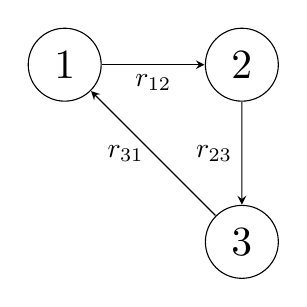
\begin{tikzpicture}[>=stealth, node distance=1.5cm]

% Define nodes
\node[circle, draw, fill=white!20, scale = 1.5] (1) {1};
\node[circle, draw, fill=white!20, scale = 1.5, right of=1] (2) {2};
\node[circle, draw, fill=white!20, scale = 1.5, below of=2] (3) {3};

% Draw edges with arrows
\draw[->] (1) -- (2) node[midway, below] {$r_{12}$};
\draw[->] (2) -- (3) node[midway, left] {$r_{23}$};
\draw[->] (3) -- (1) node[midway, left] {$r_{31}$};

% Add labels to edges (optional)


\end{tikzpicture}
\caption{A simple cyclic digraph with 3 nodes.}
\label{fig:DCG}
\end{figure}



\subsubsection{Cyclic Digraphs}

Cyclic digraphs contain no stems to generate zero rows of their graph laplacian. Additionally, if all vertices in a cyclic digraph belong to a spanning tree, only one zero eigenvalue appears. Its corresponding right eigenvector \( q \) is \( \mathbf{1}_N \) \cite{olfati-saber_consensus_2007}. The value \( k \) is arbitrary and satisfies \( p^\top \dot{x}_0 = p^\top (-Lx(0) + r) = p^\top r = v \) (since \( p^\top L = 0 \)). In the case of cyclic digraphs, \eqref{eq:0_N} is replaced by \eqref{eq:v_N}.

\begin{equation}\label{eq:v_N}
    \dot{x} \rightarrow qp^\top \dot{x}_0 = \mathbf{1}_N \times v = \mathbf{v}_N
\end{equation}

\noindent Every agent in the cyclic graph acquires a uniform velocity \( v \). This behavior is known as `velocity alignment' \cite{dimarogonas_connection_2008}. If \( v = 0 \), the system will converge and the agents will reach \( x^* \). Otherwise, the agents diverge along linear paths:

\[
x(t) = \mathbf{v}_N t + X 
\]

\noindent while \( X \) is a constant vector from integration.


Even though the system remains unstable, the distances between heads and tails become steady because \( \dot{x}_i = \dot{x}_j \). Accordingly, the difference between agent $i$ and $j$ is organized as,
\[
x_i - x_j = (vt + X_i) - (vt +X_j) = X_i-X_j
\]
%We define this invariant relative formation $X$ as the embedding result in diverging cases.

To investigate more specifically, we concentrated on \eqref{eq:total_dynamic}. As the system works for a while, all velocities will become closed to $v$. 

\begin{equation}\label{eq:findX}
\begin{split}
    \dot{x} &= k_p(Lx - r) \\
   \rightarrow  \mathbf{v}_N &= k_p(L(\mathbf{v}_Nt + X) - r) \\
           &= k_p(LX - r)  \\ \\
 \therefore X &= L^+ (r - \frac{\mathbf{v}_N}{k_p})
\end{split}
\end{equation}

Since $q=\mathbf{1}_N$ is a right eigenvector of $\lambda_1 = 0$, only $X$ has left. We determined \( X \) from \eqref{eq:findX}, where \( + \) denotes the pseudo-inverse because of \( L \)'s singularity. Followings are agent-based equations with respect to $X$:

\begin{equation}
\begin{split}
\dot{x}_i &= k_p(\sum_{j \in \mathcal{H}_i} (x_i - x_j) -r_i) \\
\rightarrow v &= k_p(\sum_{j \in \mathcal{H}_i} (X_i - X_j) - r_i) \\
X_i &= \frac{1}{|\mathcal{H}_i|}(\sum_{j \in \mathcal{H}_i} X_j +r_i-\frac{v}{k_p})
\end{split}
\end{equation}

\subsection{Bidirectional Embedding}
We got inspiration from TransE to organize directional embedding formations of knowledge graphs. Tail entities are enforced to move desired relative positions while heads receive no affection. However, we could 
reconstruct the embedding dynamics for bidirectional interaction. 
\begin{equation}
    \dot{x}_i = k_p \sum_{j \in \mathcal{N}_i} (x_i - x_j - r_{ji})
\end{equation}

We expand the range of the node's neighbors to include its tails. 

\section{Simulation}
We conducted computer simulations for embedding formulation: the acyclic digraph in Fig. \ref{fig:DAG} and the cyclic digraph in Fig. \ref{fig:DCG}. These simulations focus on how agents and their velocities change over time, providing complementary insights to our main analysis.

The embedding space is represented in $x$ and $y$ coordinates, with all entities starting from random initial positions. Since the control law \eqref{eq:fc_law} contains no nonlinear terms, the $x$ and $y$ coordinates of each agent evolve independently. %As a result, the following figures will illustrate only the changes in the $x$-coordinate for simplicity.

\begin{figure}[thb]
\begin{center}
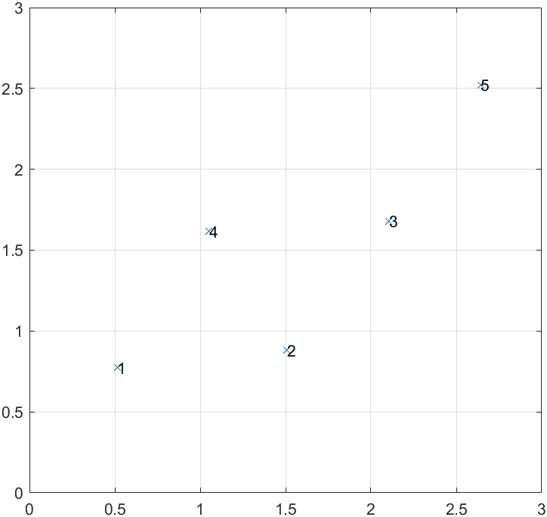
\includegraphics[width=7cm]{IMG/AG_simul3.png}
\caption{Converging acyclic digraph composed of 5 entities.}
\label{fig:DAGstate}
\end{center}
\vspace{-3mm}
\end{figure}

\begin{figure}[thb]
\begin{center}
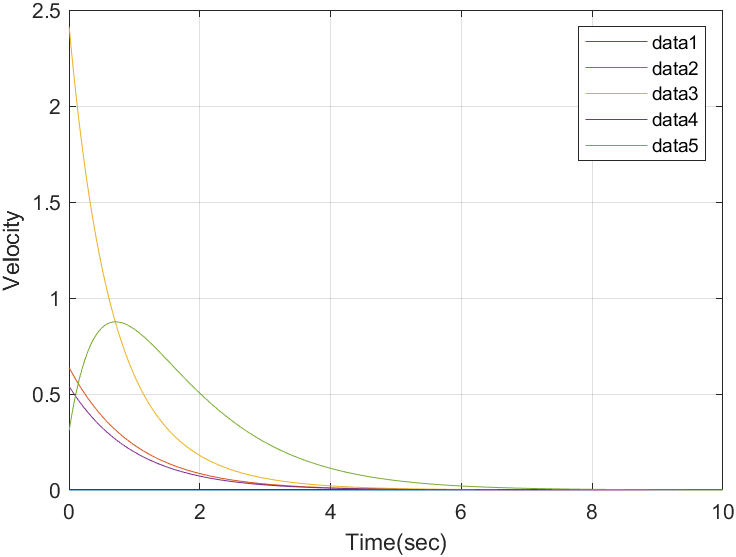
\includegraphics[width=7cm]{IMG/DAGvelocity.png}
\caption{Entities in the acyclic digraph, velocity converges to zero.}
\label{fig:DAGvelocity}
\end{center}
\vspace{-0mm}
\end{figure}

In Fig. \ref{fig:DAGstate}, the five entities have found their respective embedding points. Entity \(E_1\) retained its initial position as it is the stem node. The remaining four entities selected their positions relative to the anchor point.
\begin{equation}\label{eq:result1}
\begin{split}
    E_2 &= E_1 + r_{12}\\
    E_3 &= E_1 + \frac{r_{12}+r_{23}+r_{14}+r_{43}}{2}\\
    E_4 &= E_1 + r_{14}\\
    E_5 &= E_1 + \frac{r_{12}+r_{23}+r_{14}+r_{43}}{2} + r_{35}
\end{split}
\end{equation}

The outcome \eqref{eq:result1} accomplishes $Lx^* - r = 0$ and leads to $\dot{x} \rightarrow 0$ as illustrated in Fig. \ref{fig:DAGvelocity}. 

\begin{figure}[thb]
\begin{center}
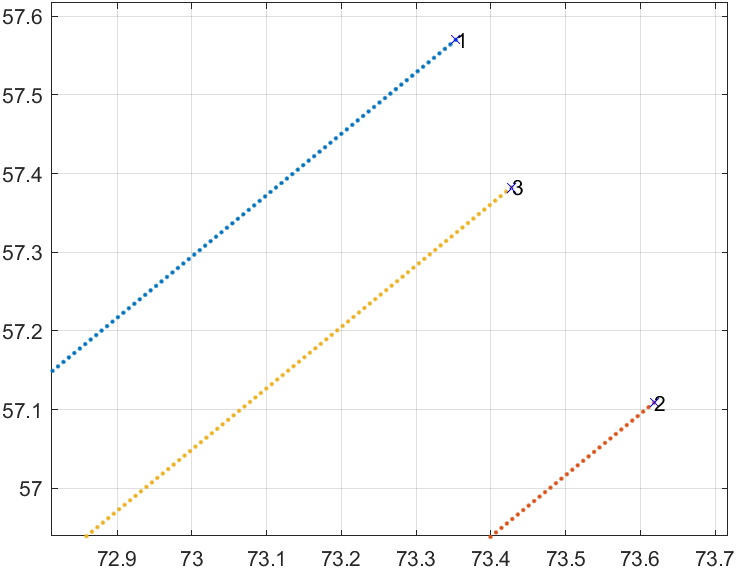
\includegraphics[width=7cm]{IMG/CG_simul3.png}
\caption{Diverging cyclic digraph composed of 3 entities at $t=10$(s).}
\label{fig:DCGstate}
\end{center}
\vspace{-3mm}
\end{figure}

\begin{figure}[thb]
\begin{center}
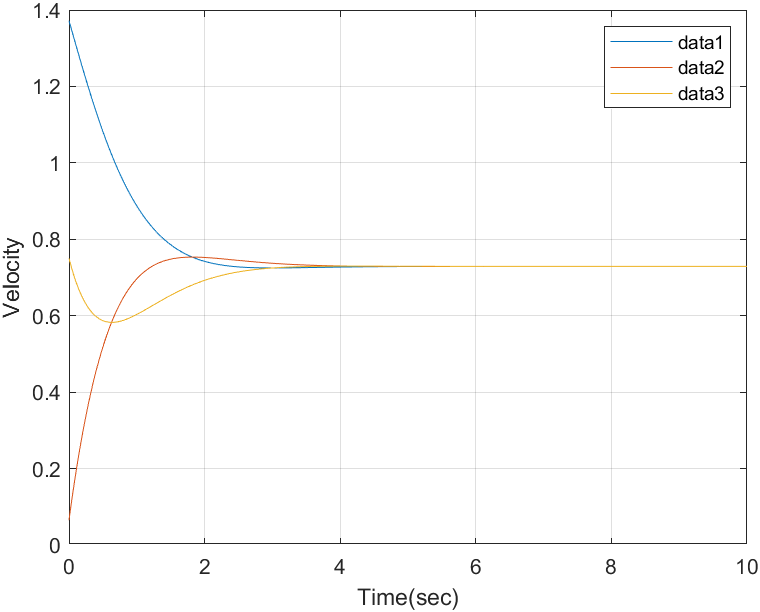
\includegraphics[width=7cm]{IMG/DCGvelocity.png}
\caption{Entities in the cyclic digraph, velocity converges to a nonzero constant.}
\label{fig:DCGvelocity}
\end{center}
\vspace{-0mm}
\end{figure}

%Figs. \ref{fig:DCGstate} and \ref{fig:DCGvelocity} represent the embedding of the cyclic digraph. Entities continue to move, as they cannot realize zero-gradient locations according to \eqref{eq:\mathbf{v}_N}. 

\section{Conclusion}
In this paper, we have proposed a novel integration of Knowledge Graph Embedding (KGE) with distributed optimization and formation control. 
By reformulating the TransE optimization problem as a distributed optimization task, we demonstrated how multi-agent systems can effectively learn embeddings while interacting only with neighboring entities. 
This approach leverages graph-theoretical concepts, specifically the properties of the graph Laplacian, to analyze the convergence and stability of the embedding process.
Our results highlight that TransE, when interpreted through the lens of distributed optimization, can be seen as a formation control problem. 
The equivalence between the gradient descent dynamics in distributed optimization and the control laws in formation control allows for a deeper understanding of the embedding process in multi-agent systems.
The use of the in-degree Laplacian matrix \(L\) provides valuable information on the stability and convergence behavior of the embedding.
Overall, this work bridges the gap between knowledge graph embedding, distributed optimization, and formation control, offering a comprehensive framework for understanding and improving the performance of KGE methods in decentralized and multi-agent environments.


\bibliographystyle{IEEEtran}
\bibliography{kge}

\end{document}


% \begin{figure}[thb]
% \begin{center}
% 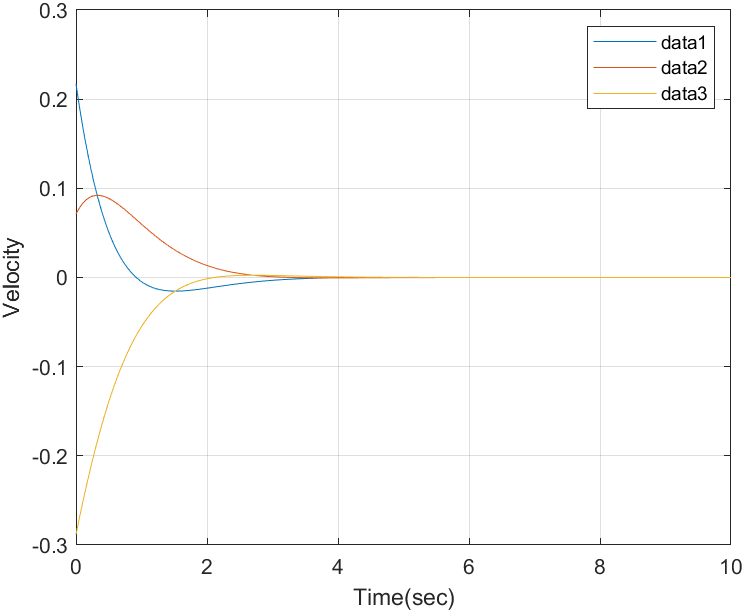
\includegraphics[width=7cm]{IMG/DCG_0.png}
% \caption{Velocities converge to 0 in the DCG.}
% \label{fig:DCG_0}
% \end{center}
% \vspace{-7mm}
% \end{figure}

% DCGs have no stem nodes similar to Fig. \ref{fig:DCG}, so \( L \) has no zero rows. 
% This difference makes it impossible for DCGs to satisfy the Lemma \ref{lemma:p}. 
% Therefore, DCG convergence is quite a special case, as \( p \), \( q \), and \( \dot{x}_0 \) should appropriately match \( qp^\top \dot{x}_0 = \mathbf{0}_N \).

% \begin{figure}[thb]
% \begin{center}
% 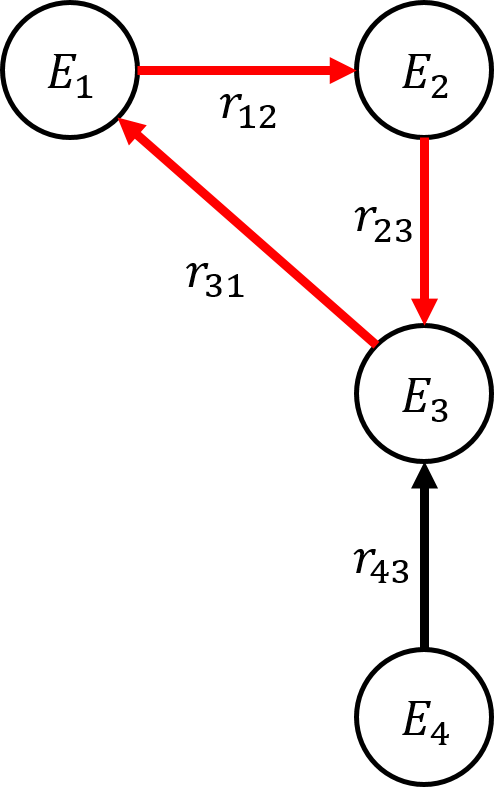
\includegraphics[width=5cm]{IMG/AG1.png}
% \caption{An acyclic digraph with 4 nodes. The cycle has a direct stem.}
% \label{fig:AG1}
% \end{center}
% \vspace{-0mm}
% \end{figure}


% \begin{figure}[thb]
% \begin{center}
% 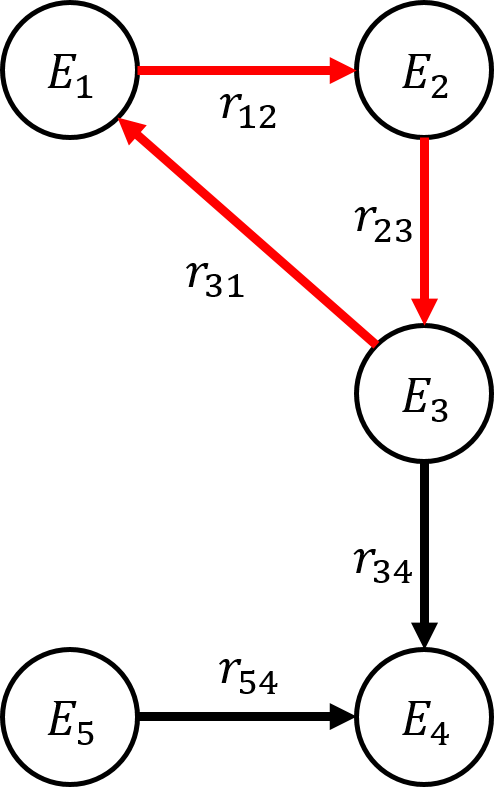
\includegraphics[width=5cm]{IMG/GG1.png}
% \caption{A general digraph with 5 nodes. One stem and one cycle.}
% \label{fig:GG1}
% \end{center}
% \vspace{-0mm}
% \end{figure}

% \begin{figure}[thb]
% \begin{center}
% 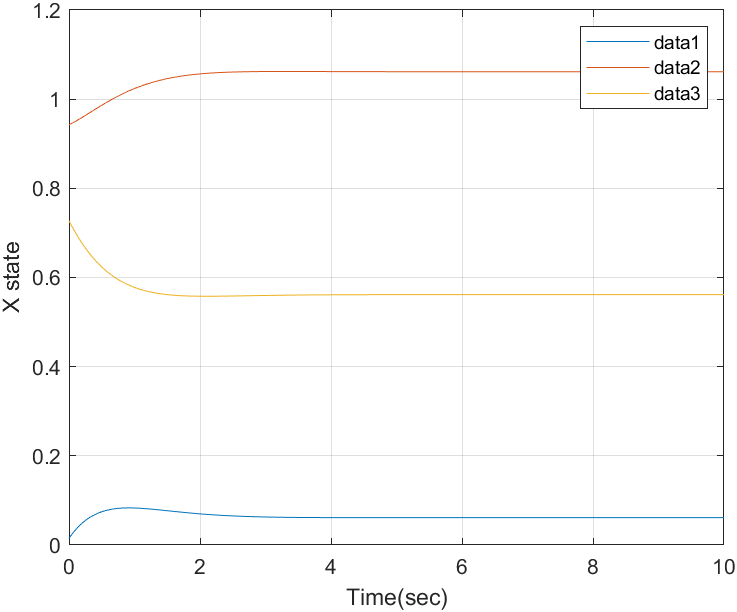
\includegraphics[width=7cm]{IMG/DCGsettle.png}
% \caption{Converging entities in the DCG.}
% \label{fig:DCGsettle}
% \end{center}
% \vspace{-3mm}
% \end{figure}

% \begin{tikzpicture}
% \node[mynode](n3) at (0,0){3};
% \node[mynode](n2) at (132:3){2};
% \node[mynode](n4) at (204:3){4};
% \node[mynode](n5) at (276:3){5};
% \node[mynode](n1) at (168:5){1};
% \draw[myarrow](n1)--(n4);
% \draw[myarrow](n1)--(n2);
% \draw[myarrow](n2)--(n3);
% \draw[myarrow](n4)--(n3);
% \draw[myarrow](n3)--(n5);
% \end{tikzpicture}


% \begin{thebibliography}{99}

%     \bibitem{bordes2013transe}
%     Bordes, A., Usunier, N., Garcia-Duran, A., Weston, J., and Yakhnenko, O. (2013). Translating embeddings for modeling multi-relational data. Advances in neural information processing systems, 26.
    
%     \bibitem{saber2007consensus}
%     Olfati-Saber, R., Fax, J. A., and Murray, R. M. (2007). Consensus and cooperation in networked multi-agent systems. Proceedings of the IEEE, 95(1), 215-233.
    
%     \bibitem{wang2017knowledge}
%     Wang, Q., Mao, Z., Wang, B., and Guo, L. (2017). Knowledge graph embedding: A survey of approaches and applications. IEEE transactions on knowledge and data engineering, 29(12), 2724-2743.
    
%     \bibitem{oh2015survey}
%     Oh, K. K., Park, M. C. and Ahn, H. S. (2015). A survey of multi-agent formation control. Automatica, 53, 424-440.
    
%     \bibitem{dimaro2008alignment}
%     Dimarogonas, D. V. and Kyriakopoulos, K. J. (2008). A connection between formation infeasibility and velocity alignment in kinematic multi-agent systems. Automatica, 44, 2648-2654.
    
%     \bibitem{yang2019survey}
%     Yang, T., \textit{et al.} (2019). A survey of distributed optimization. Annual reviews in control, 47, 278-305.
    
%     \bibitem{mir2013lap}
%     Mirzaev, I., and Gunawardena, J. (2013). Laplacian dynamics on general graphs. Bulletin of mathematical biology, 75(11), 2118-2149.
    
%     \bibitem{nedic2009subgrad}
%     Nedic, A., and Ozdaglar, A. (2009). Distributed subgradient methods for multi-agent optimization. IEEE Transactions on Automatic Control, 54(1), 48-61.
    
%     % \bibitem{ma2024cluster}
%     % Ma, J. M., \textit{et al.} (2024). Topological approach and analysis of clustering in consensus networks. Systems \& Control Letters, 183, 105699.
    
%     \end{thebibliography}